% generated by scripts/pkl_to_latex.py
% source PKL : thermal_v1_L8_Ne8_U10_t1_mode-uniform_tpall_t2all_tperpall_nmin2_solver-gcg_full_restarts8_iter200_kmax4_tol1em09_cut10_adaptive1_step5_clusteravg1_T0to1_N20-148a4f8ecb18_knone_diag0.pkl
% scan type  : Tscan
% state      : gs
% requires   : \usepackage{pgfplots} \pgfplotsset{compat=1.18}
% colours match the matplotlib PDF (tab10 cycle)
\definecolor{gmeC0}{HTML}{1F77B4}
\definecolor{gmeC1}{HTML}{FF7F0E}
\definecolor{gmeC2}{HTML}{2CA02C}
\definecolor{gmeC3}{HTML}{D62728}
\definecolor{gmeC4}{HTML}{9467BD}
\definecolor{gmeC5}{HTML}{8C564B}
\definecolor{gmeC6}{HTML}{E377C2}
\definecolor{gmeC7}{HTML}{17BECF}

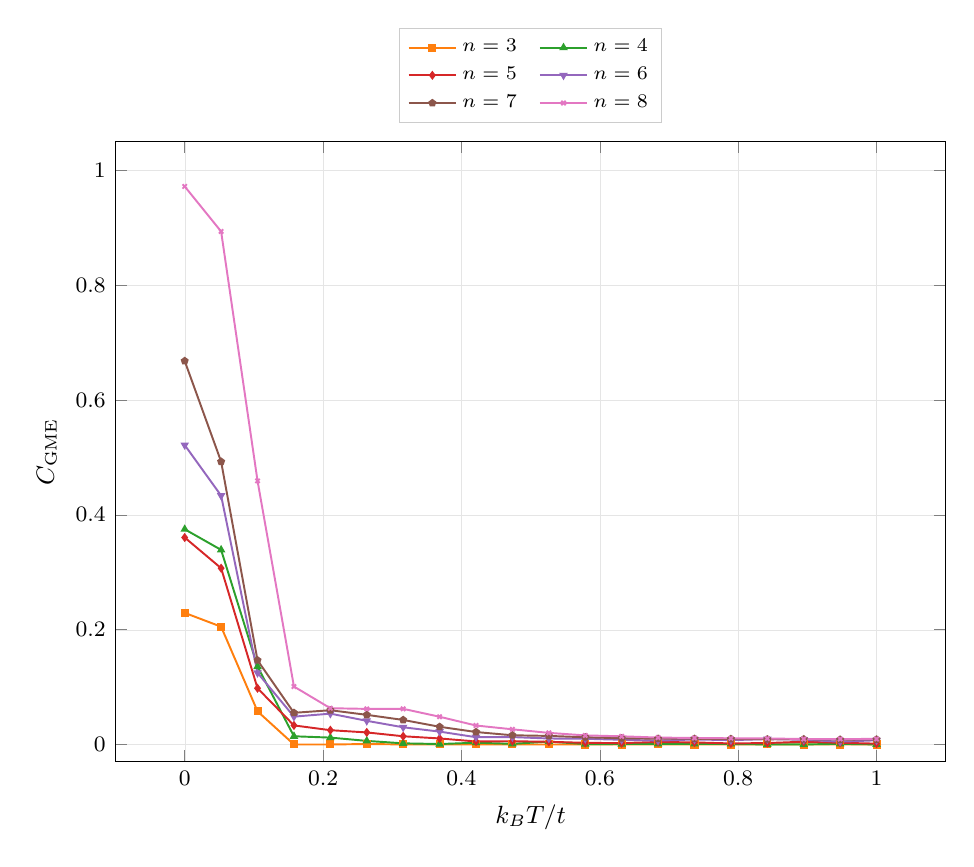
\begin{tikzpicture}
  \begin{axis}[
    width=\columnwidth,
    height=0.78\columnwidth,
    xlabel={$k_B T/t$},
    ylabel={$C_{\mathrm{GME}}$},
    grid=both,
    grid style={line width=.1pt, draw=gray!20},
    tick label style={font=\footnotesize\rmfamily, /pgf/number format/fixed},
    label style={font=\small\rmfamily},
    scaled ticks=false,
    legend style={font=\scriptsize\rmfamily, draw=gray!40, at={(0.5,1.03)}, anchor=south, /tikz/every even column/.append style={column sep=6pt}},
    legend cell align={left},
    legend columns=2,
    ymin=-0.03,
    ymax=1.05,
  ]
    \addplot[color=gmeC1, mark=square*, mark size=1.1pt, line width=0.7pt] coordinates {
        (0,0.229253) (0.052632,0.205165) (0.105263,0.057789) (0.157895,0.000052)
        (0.210526,0.000081) (0.263158,0.000824) (0.315789,0.000181) (0.368421,0.000252)
        (0.421053,0.000188) (0.473684,0.000048) (0.526316,0.000083) (0.578947,0.000039)
        (0.631579,0.000024) (0.684211,0.000198) (0.736842,0.000012) (0.789474,0.000009)
        (0.842105,0.000055) (0.894737,0.000023) (0.947368,0.000011) (1,0.00003)
    };
    \addlegendentry{$n=3$}
    \addplot[color=gmeC2, mark=triangle*, mark size=1.1pt, line width=0.7pt] coordinates {
        (0,0.374877) (0.052632,0.33892) (0.105263,0.135744) (0.157895,0.01435)
        (0.210526,0.012035) (0.263158,0.006308) (0.315789,0.002037) (0.368421,0.000858)
        (0.421053,0.003099) (0.473684,0.001164) (0.526316,0.005064) (0.578947,0.000778)
        (0.631579,0.000861) (0.684211,0.001061) (0.736842,0.001012) (0.789474,0.000912)
        (0.842105,0.000156) (0.894737,0.000142) (0.947368,0.001121) (1,0.000176)
    };
    \addlegendentry{$n=4$}
    \addplot[color=gmeC3, mark=diamond*, mark size=1.1pt, line width=0.7pt] coordinates {
        (0,0.360457) (0.052632,0.307059) (0.105263,0.09797) (0.157895,0.033265)
        (0.210526,0.024929) (0.263158,0.021052) (0.315789,0.014369) (0.368421,0.010547)
        (0.421053,0.005309) (0.473684,0.005738) (0.526316,0.004736) (0.578947,0.00291)
        (0.631579,0.002425) (0.684211,0.004456) (0.736842,0.003664) (0.789474,0.001868)
        (0.842105,0.002578) (0.894737,0.00486) (0.947368,0.002985) (1,0.00155)
    };
    \addlegendentry{$n=5$}
    \addplot[color=gmeC4, mark=triangle*, mark size=1.1pt, mark options={rotate=180}, line width=0.7pt] coordinates {
        (0,0.521493) (0.052632,0.433422) (0.105263,0.124803) (0.157895,0.048543)
        (0.210526,0.053764) (0.263158,0.041259) (0.315789,0.029991) (0.368421,0.022475)
        (0.421053,0.012739) (0.473684,0.01292) (0.526316,0.010487) (0.578947,0.009965)
        (0.631579,0.008263) (0.684211,0.00672) (0.736842,0.008797) (0.789474,0.007622)
        (0.842105,0.009392) (0.894737,0.008319) (0.947368,0.004888) (1,0.00736)
    };
    \addlegendentry{$n=6$}
    \addplot[color=gmeC5, mark=pentagon*, mark size=1.1pt, line width=0.7pt] coordinates {
        (0,0.667931) (0.052632,0.492642) (0.105263,0.146674) (0.157895,0.055197)
        (0.210526,0.0597) (0.263158,0.051667) (0.315789,0.042785) (0.368421,0.030891)
        (0.421053,0.021751) (0.473684,0.016094) (0.526316,0.014981) (0.578947,0.012612)
        (0.631579,0.01089) (0.684211,0.010139) (0.736842,0.01003) (0.789474,0.009707)
        (0.842105,0.009075) (0.894737,0.009285) (0.947368,0.00859) (1,0.008804)
    };
    \addlegendentry{$n=7$}
    \addplot[color=gmeC6, mark=x, mark size=1.1pt, line width=0.7pt] coordinates {
        (0,0.97189) (0.052632,0.893417) (0.105263,0.459098) (0.157895,0.101001)
        (0.210526,0.063185) (0.263158,0.062051) (0.315789,0.062137) (0.368421,0.048346)
        (0.421053,0.03309) (0.473684,0.026487) (0.526316,0.020257) (0.578947,0.015888)
        (0.631579,0.014306) (0.684211,0.012107) (0.736842,0.01139) (0.789474,0.010854)
        (0.842105,0.010492) (0.894737,0.009659) (0.947368,0.009606) (1,0.009696)
    };
    \addlegendentry{$n=8$}
  \end{axis}
\end{tikzpicture}
